\section*{Problem 10}


$$
\begin{array}{l}
\dot{x}_{1}=x_{2} \\
\dot{x}_{2}=-x_{1}+\frac{1}{3} x_{1}^{3}-x_{2}
\end{array}
$$


In order to determine the equilibrium points of the system we must set the state equations equal and solve.

$$
\begin{array}{l}
0=x_{2} \\
0=-x_{1}+\frac{1}{3} x_{1}^{3}-x_{2}
\end{array}
$$


\noindent Therefore we can show that since $x_2 =0$ , we can solve for the remaining values of $x_1$, such that..

$$
x_1^2 = 3
$$

\noindent This yields the following solutions.

\begin{enumerate}
  \item \textbf{Eq. Pt. \#1:} $x_1=x_2 =0$
  \item \textbf{Eq. Pt. \#2:} $x_2=0$ and $x_1 = \sqrt{3}$
  \item \textbf{Eq. Pt. \#3:}  $x_2=0$ and $x_1 = -\sqrt{3}$

\end{enumerate}


\subsection*{Contour Plots }

Given the Lyapunov Candidate function $V(x)=\frac{3}{4} x_{1}^{2}-\frac{1}{12} x_{1}^{4}+\frac{1}{2} x_{1} x_{2}+\frac{1}{2} x_{2}^{2}$, we want to show graphically the region of attraction and that this point is only \underline{stable} when $V(x)< \frac{9}{8} < 1.125$.


\begin{center}
  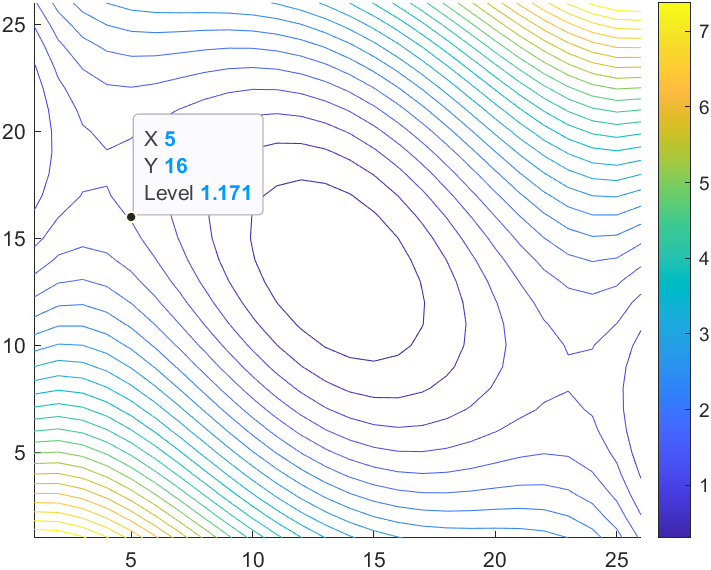
\includegraphics[scale=.65]{Lyapunov_Contour_prob10}
\end{center}


\noindent We can see in the contour plot that the trajectory of the system greater than $1.125$ will not converge to the origin , but will be attracted to other points in the system.
